\subsection{Diagramas de dispersión e interpretación}
\subsubsection*{Datos, ejes y control de completitud}
Se usa IMERG Final V07B promediado por área sobre el polígono exacto de La Vieja, no el promedio histórico de caja. Eje horizontal: precipitación acumulada mensual (mm/mes); eje vertical: lluvia local (mm/mes), caudal medio mensual Q (m$^3$/s) o escorrentía R (mm/mes), según el panel. Los colores identifican los doce meses calendario. IMERG--Q usa 285 meses completos entre enero de 1998 y diciembre de 2022. Zaragoza-AUT solo aporta 14 meses completos entre enero de 2018 y agosto de 2019. El archivo tiene 22 acumulados no vacíos, pero ocho son parciales: se excluyen porque sus intervalos registrados no alcanzan los esperados. No se rellenan ni prorratean datos. Estos conteos y la serie poligonal sustituyen las cifras históricas de este apartado.
\begin{figure}[H]\centering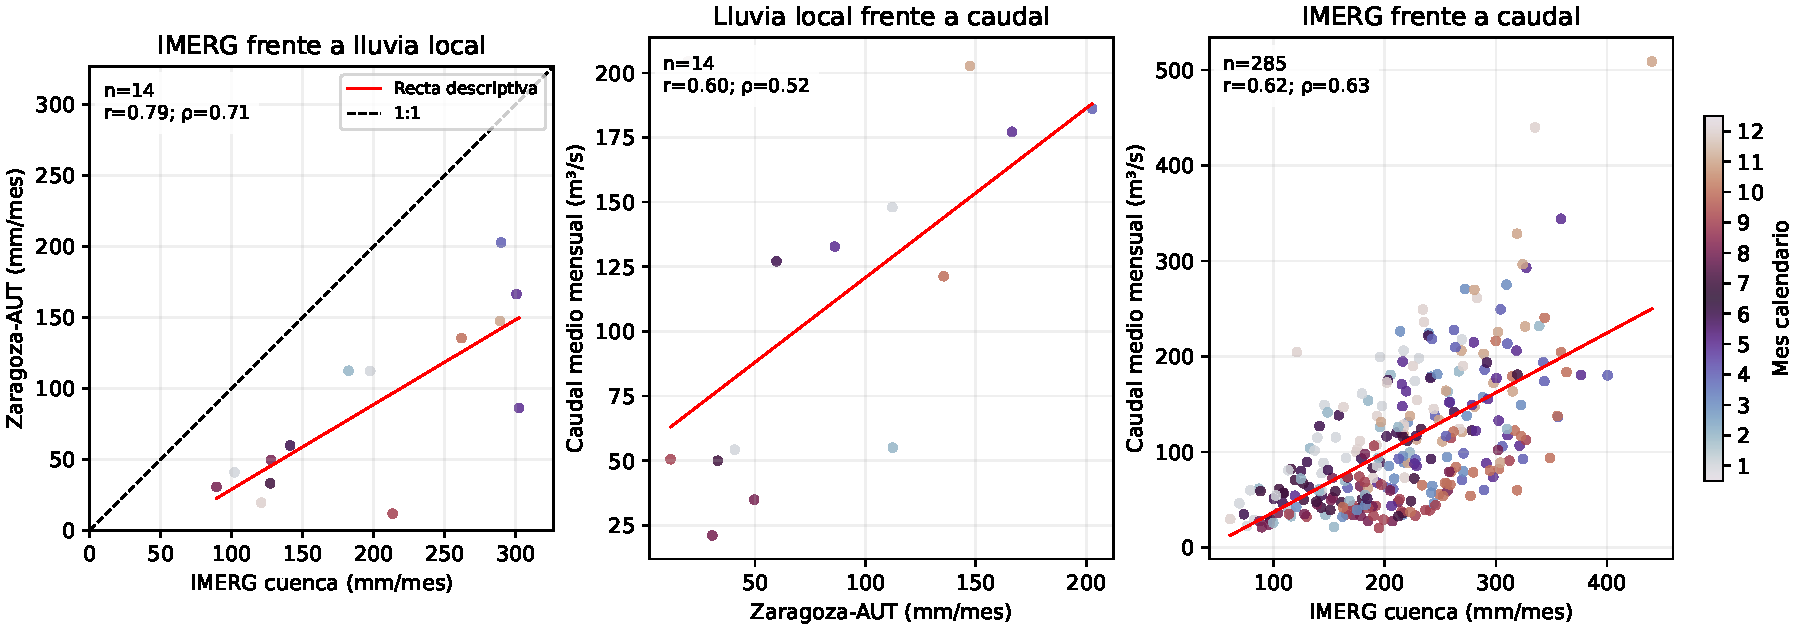
\includegraphics[width=\linewidth]{../apartado_2_1/dispersiones_21.pdf}\caption{Tres diagramas requeridos con IMERG de polígono y lluvia local completa.}\end{figure}
\begin{figure}[H]\centering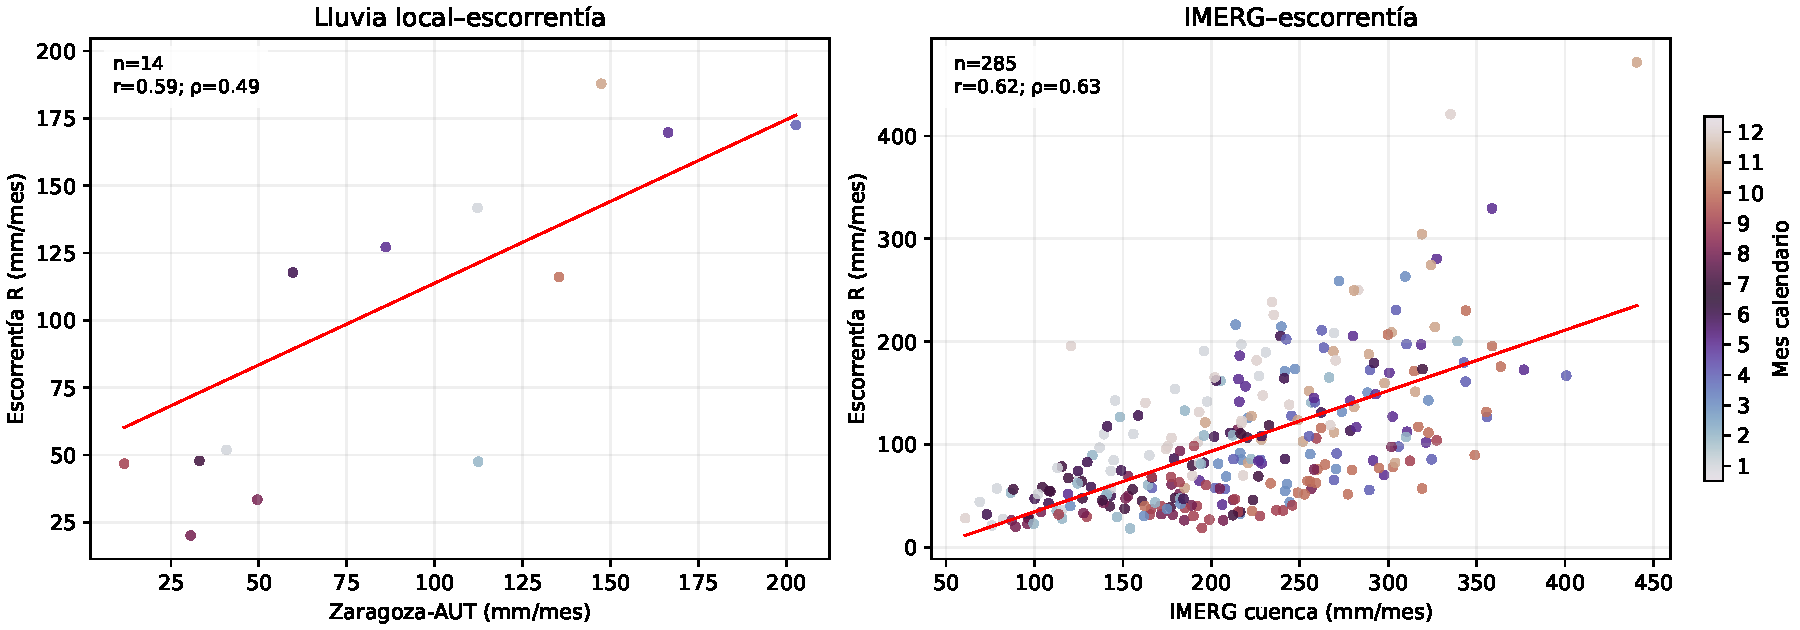
\includegraphics[width=\linewidth]{../apartado_2_1/laminas_21.pdf}\caption{Comparación de precipitación y escorrentía en láminas mensuales.}\end{figure}
\subsubsection*{Dirección, forma, dispersión y agrupamientos}
Las tres nubes muestran asociación positiva; IMERG--lluvia local es la más fuerte en la muestra pequeña, mientras lluvia local--Q e IMERG--Q son moderadas. La nube IMERG--Q es alargada y dispersa, sin una función única: una misma lluvia puede acompañarse de caudales diferentes. Los meses calendario se solapan; el color ayuda a detectar agrupamientos estacionales, pero no establece regímenes separados. No hay soporte para ajustar curvaturas con solo 14 puntos locales. Se observan puntos de Q alto fuera del núcleo de la nube; una mayor amplitud a magnitudes altas puede sugerir variabilidad dependiente de la magnitud, pero no constituye una prueba de heterocedasticidad.
\subsubsection*{Sesgo, MAE y RMSE frente a la referencia local}
La línea 1:1 usa límites y escalas iguales. Con lluvia local como referencia y error e = IMERG - local, el sesgo medio es +109,80 mm/mes, MAE 109,80 mm/mes y RMSE 119,61 mm/mes (n=14). El sesgo indica la diferencia media con signo; MAE mide la diferencia absoluta típica; RMSE da más peso a errores grandes. Todos los errores de esta muestra son positivos, por eso sesgo y MAE coinciden. IMERG es un promedio de cuenca y Zaragoza una medición puntual: la diferencia combina representatividad espacial, cobertura y errores de ambas fuentes; no es una validación contra la lluvia verdadera de toda la cuenca. Una correlación alta no garantiza concordancia con 1:1.
\subsubsection*{Pearson, Spearman y valores influyentes}
Pearson resume asociación lineal y es sensible a magnitudes extremas; Spearman correlaciona rangos y resume asociación monótona. Sus diferencias no prueban por sí solas no linealidad. Se comprueba influencia retirando un mes cada vez: la tabla de sensibilidad muestra el mes que más cambia Pearson y el intervalo obtenido. No se eliminan extremos del análisis. Noviembre y diciembre de 2010 destacan por caudales altos en IMERG--Q; diciembre de 2018 combina poca lluvia local y caudal alto, compatible con lluvia antecedente o aportes de otras zonas. Son hipótesis de interpretación que requieren datos adicionales, no causas demostradas.
\begin{center}\small\begin{tabular}{lrrr}\hline
Relación & n & Pearson & Spearman \\ \hline
IMERG--lluvia local & 14 & 0,79 & 0,71 \\
Lluvia local--caudal & 14 & 0,60 & 0,52 \\
IMERG--caudal & 285 & 0,62 & 0,63 \\
IMERG--escorrentía & 285 & 0,62 & 0,63 \\
\hline\end{tabular}\end{center}
\begin{center}\small\begin{tabular}{lrrrr}\hline
Relación & Mes influyente & r sin mes & r mínimo & r máximo \\ \hline
IMERG--lluvia local & 2018-09 & 0,87 & 0,75 & 0,87 \\
Lluvia local--caudal & 2018-12 & 0,84 & 0,53 & 0,84 \\
IMERG--caudal & 2010-11 & 0,60 & 0,60 & 0,63 \\
IMERG--escorrentía & 2010-11 & 0,60 & 0,60 & 0,63 \\
\hline\end{tabular}\end{center}
\subsubsection*{Rezagos mensuales y apoyo con láminas}
Se define k$\geq$0 como correlación entre P del mes t-k y Q del mes t; k=1 significa lluvia del mes anterior. Se preserva el calendario mensual antes de desplazar, para no saltar faltantes. Se exploran 0--3 meses por posible humedad antecedente y almacenamiento; no se invocan nieve ni regulación documentada para explicar esta cuenca. Nunca se usa lluvia futura para explicar caudal pasado. Las muestras cambian por disponibilidad: los máximos de correlación son descriptivos y no estiman automáticamente un tiempo físico de respuesta. La comparación en láminas usa R = 86,4 $\times$ días del mes $\times$ Q / 2797,19, en mm/mes. R deriva de Q y no aporta evidencia independiente; sus diferencias mensuales incluyen la duración del mes. Los diagramas P--R ayudan a comparar unidades, pero no cierran un balance hídrico sin evapotranspiración y almacenamiento. En IMERG--Q, Pearson original es mayor sin rezago (0,62), mientras Spearman es ligeramente mayor a un mes (0,65 frente a 0,63): no hay un único rezago óptimo independiente del indicador. Con anomalías, el mayor valor de ambas correlaciones ocurre sin rezago (Pearson 0,64; Spearman 0,60). Para lluvia local--Q el máximo explorado es un mes (Pearson 0,65; Spearman 0,64), pero solo hay 14 pares y las muestras cambian. La correlación negativa a tres meses puede mezclar estacionalidad y tamaño muestral; no demuestra una respuesta física inversa.
\textbf{Rezagos: original.} $P(t-k)$ frente a $Q(t)$ o $R(t)$.
\begin{center}\small\begin{tabular}{lrrrr}\hline
Relación & k & n & Pearson & Spearman \\ \hline
Lluvia local--caudal & 0 & 14 & 0,60 & 0,52 \\
Lluvia local--caudal & 1 & 14 & 0,65 & 0,64 \\
Lluvia local--caudal & 2 & 14 & 0,14 & 0,09 \\
Lluvia local--caudal & 3 & 14 & -0,43 & -0,43 \\
IMERG--caudal & 0 & 285 & 0,62 & 0,63 \\
IMERG--caudal & 1 & 284 & 0,60 & 0,65 \\
IMERG--caudal & 2 & 283 & 0,32 & 0,36 \\
IMERG--caudal & 3 & 282 & 0,08 & 0,06 \\
IMERG--escorrentía & 0 & 285 & 0,62 & 0,63 \\
IMERG--escorrentía & 1 & 284 & 0,60 & 0,66 \\
IMERG--escorrentía & 2 & 283 & 0,32 & 0,36 \\
IMERG--escorrentía & 3 & 282 & 0,07 & 0,06 \\
\hline\end{tabular}\end{center}
\textbf{Rezagos: anomalia.} $P(t-k)$ frente a $Q(t)$ o $R(t)$.
\begin{center}\small\begin{tabular}{lrrrr}\hline
Relación & k & n & Pearson & Spearman \\ \hline
IMERG--caudal & 0 & 285 & 0,64 & 0,60 \\
IMERG--caudal & 1 & 284 & 0,50 & 0,50 \\
IMERG--caudal & 2 & 283 & 0,41 & 0,44 \\
IMERG--caudal & 3 & 282 & 0,43 & 0,46 \\
IMERG--escorrentía & 0 & 285 & 0,63 & 0,60 \\
IMERG--escorrentía & 1 & 284 & 0,50 & 0,50 \\
IMERG--escorrentía & 2 & 283 & 0,41 & 0,44 \\
IMERG--escorrentía & 3 & 282 & 0,42 & 0,45 \\
\hline\end{tabular}\end{center}
\subsubsection*{Anomalías y persistencia al retirar el ciclo anual}
Se define X'(t)=X(t)-promedio de X para el mes calendario de t. Para I, Q y R se calcula una climatología común de enero de 1998--diciembre de 2022 usando exclusivamente los 285 meses simultáneos completos; el archivo de climatología conserva el conteo por mes. La misma definición deberá utilizarse al integrar los apartados 1.5 y 3.2. La asociación IMERG--Q persiste después de retirar el ciclo anual: se reportan Pearson y Spearman de las anomalías y sus rezagos. Esto indica asociación entre desviaciones respecto de lo habitual, sin demostrar causalidad ni capacidad predictiva. No se presenta una climatología local como confiable: Zaragoza tiene solo 14 meses válidos, marzo no tiene ninguno y varios meses tienen un solo año. No es defendible completar la comparación de anomalías de las dos parejas locales con esa cobertura; se necesitan más años de lluvia local verificada. Sin rezago, las anomalías IMERG--Q dan Pearson 0,64 y Spearman 0,60.
\begin{figure}[H]\centering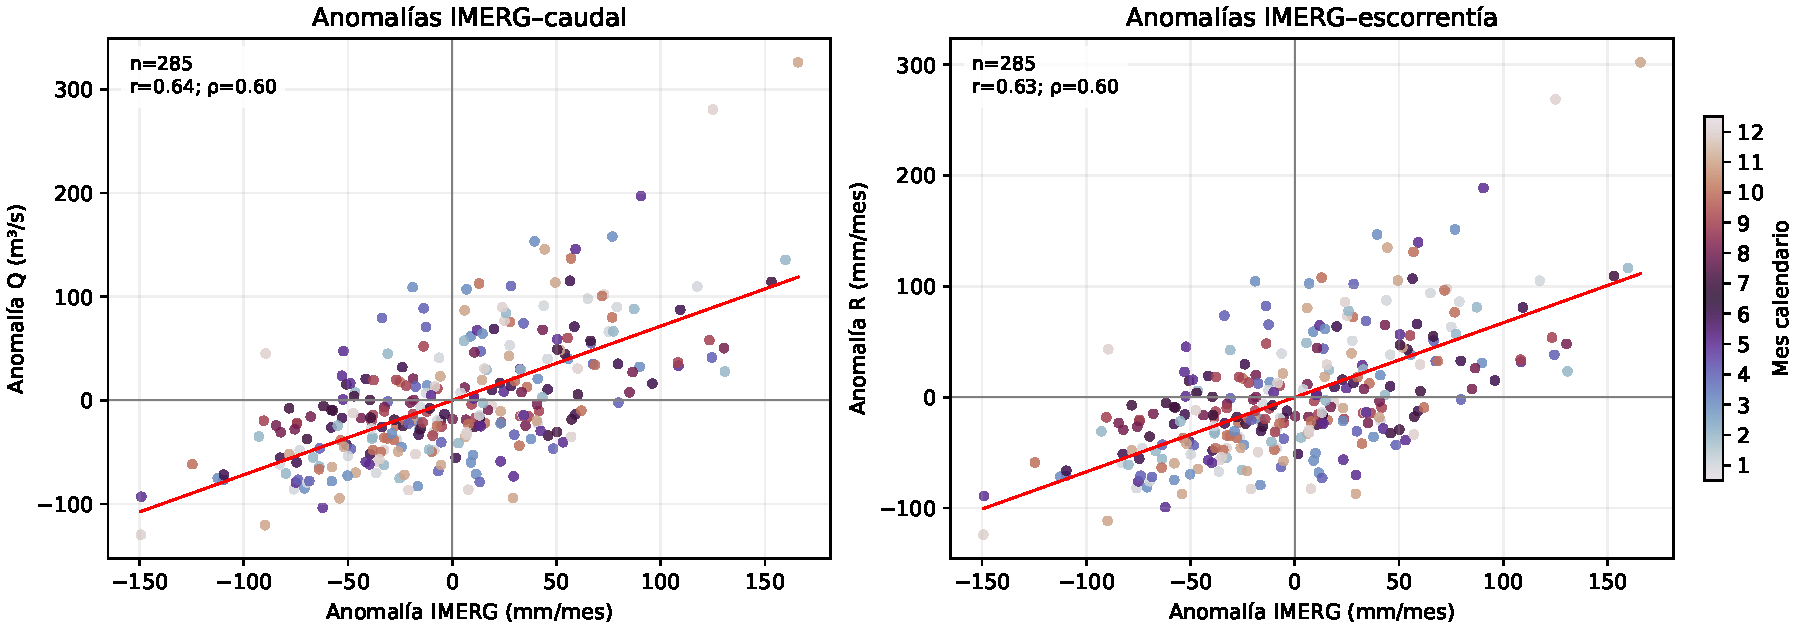
\includegraphics[width=\linewidth]{../apartado_2_1/anomalias_21.pdf}\caption{Anomalías con climatología común 1998--2022.}\end{figure}
\subsubsection*{Alcance del apartado}
Quedan desarrollados los tres diagramas, sus ejes y colores, los errores frente a lluvia local, ambas correlaciones, la sensibilidad a puntos influyentes, los rezagos y la comparación de anomalías IMERG--Q con apoyo P--R. La comparación de anomalías que incluye lluvia local queda condicionada a obtener una climatología adecuada. No se calculan p-valores simples suponiendo meses independientes, ni se atribuye causalidad. Una evaluación predictiva necesita separación temporal de ajuste y validación, prevista en 2.2 y 2.3.
